\section{Introduction}
This report deals with the implementation of a  vending 
machine control circuit, made to run on a Basys2 FPGA board. When implemented,
a user will be able to simulate normal use of a real vending machine, by use of the onboard toggleswitches and pushbuttons.

\begin{figure}
    \center
    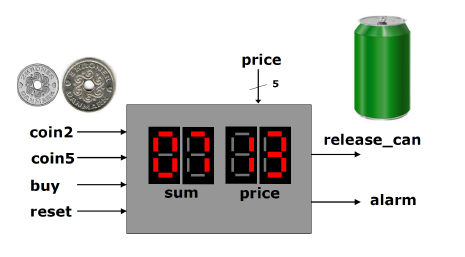
\includegraphics{pictures/vending_interface.png}
    \caption{Illustration of the vending machine interface, from the exercise manual}
    \label{vending_interface}
\end{figure}

As can be seen on figure \ref{vending_interface}, the vending machine accepts
2kr and 5kr coins, and uses the 7-segment display on the Basys2 board to show
how much money is currently avaible for a purchase as well as the price of a soda.
To indicate that a can of soda has been dispensed by the machine, an LED will light up. Should there not be enough money for a purchase, an alarm LED will light up.
A more detailed description of how the machine operates can be found in the specifications section. \\

We have chosen to implement the vending machine controller circuit, on the FPGA, in two different ways.
First by creating a fixed controller with a corresponding datapath, connected to a 7-segment display driver,
and second, by developing a simple 8-bit microprocessor that can run a vending machine program written in assembly language.

Because of this, this report will be split into 2 parts. One which covers the datapath/controller approach
and one which covers the microprocessor approach.

\subsection{Project Specification}
The finished vending machine controller must support the following actions

\begin{itemize}
    \item User defined \textbf{price} which is set as a binary number using 5 toggle switches.
    \item The price must be visible on the 7-segment display
    \item The machine accepts 2kr and 5kr coins, emulated by 2 push buttons called \textbf{coin2} and \textbf{coin5}
    \item The amount of money available for the current transaction is called \textbf{sum} and is visible on the 7-segment display.
    \item A pushbutton called \textbf{buy} can be pressed.
    \item If there is enough money in the machine to conduct a purchase and \textbf{buy} is pressed, the signal, \textbf{release\_can}, is asserted until \textbf{buy} is no longer pressed.
    \item If there is not enough money in the machine and \textbf{buy} is pressed, the signal, \textbf{alarm}, is asserted until \textbf{buy} is no longer pressed.
    \item Asserting the \textbf{reset} signal, will reset the machine to it's initial configuration, where it is full of cans, empty of coins, and the \textbf{sum} is 0.
    \item The machine cannot return any money. Leftover coins from a purchase are left in the machine for the next purchase.

\end{itemize}

Furthermore, normal operation of the machine assumes that

\begin{itemize}
    \item The system runs on a 763Hz clock.
    \item The system can be run on a manual clock, selectable with the pushbutton \textbf{sel\_man}.
    \item The user never enters more money than the machine can handle.
    \item The vending machine never runs out of cans.
    \item Only one input signal, excluding \textbf{price}, is asserted at any one time.
    \item The machine uses a hexadecimal display for showing \textbf{price} and \textbf{sum}
    \item Inputs are asynchronous and need to be synchronized.
\end{itemize}
We have chosen to implement a decimal display instead of the hexadecimal display in both the controller/datapath implementation and the microprocessor implementation.
In the microprocessor implementation we have also included the possibility of the machine running out of cans, together with detection of full coin compartments.

